% https://tex.stackexchange.com/questions/27351/speed-up-beamer-compile-time

\documentclass[xcolor={dvipsnames,table},aspectratio=169]{beamer}
% \includeonlyframes{current}

\graphicspath{{graphics/}}

\title{Reviving the Media Station:\\A Study in Reverse Engineering}
\author{Nathanael Gentry}
\institute{School of Engineering}
\date{April 13, 2021}

\usepackage{listings}
\lstset{basicstyle=\ttfamily, keywordstyle=\bfseries, language=Python, escapeinside={(*}{*)}}

\usepackage{amsmath}
\usepackage{lmodern}

% https://tex.stackexchange.com/questions/107042/beamer-overlay-box-around-text-the-correct-way
% \usetikzlibrary{calc}
% \newcommand{\tikzmark}[1]{\tikz[overlay,remember picture] \node (#1) {};}

\usepackage{tikz}
\usetikzlibrary{decorations.pathreplacing,calc,shapes,positioning,tikzmark}
% \newcommand\tbox[1]{\tikz[baseline]{\node[inner sep=2pt, draw=red, ultra thick, anchor=text, rectangle] {#1};}}

% https://stackoverflow.com/questions/1346512/to-escape-many-in-latex-efficiently
\usepackage{underscore}

\usepackage[T1]{fontenc}
\usepackage{caption}

\usepackage{forest}
\usepackage{bytefield}

\usepackage{verbatim}
\usepackage{fancyvrb}
\fvset{listparameters=\setlength{\topsep}{0pt}\setlength{\partopsep}{0pt}}

\usepackage{colortbl}
\newlength{\dumpcolsep}
\setlength{\dumpcolsep}{1.5em}
\setlength{\tabcolsep}{0pt}
\newcolumntype{C}[1]{@{}>{\centering\arraybackslash}p{#1}@{}}
\newcolumntype{D}{@{}>{\centering\arraybackslash}p{\dumpcolsep}@{}}

\newcommand{\hexdump}[3]{
  {\ttfamily
  \begin{tabular}{C{2.5em}|@{\hspace{0.1em}}*{16}{D}@{}|@{\hspace{0.35em}}*{16}{C{0.57em}}}
    \input{dumps/#1}
  \end{tabular}}
\source{\cite{#2}, \texttt{#3} }
}

% https://tex.stackexchange.com/questions/5073/making-a-simple-directory-tree
\forestset{%
  default preamble={for tree={%
      font=\ttfamily\LARGE, %
      grow'=0, %
      child anchor=west, %
      parent anchor=south, %
      anchor=west, %
      calign=first, %
      edge path={ %
        \noexpand\path [draw, \forestoption{edge}] %
        (!u.south west) +(7.5pt,0) |- node[fill,inner sep=1.25pt] {} (.child anchor)\forestoption{edge label}; %
      }, %
      before typesetting nodes={ %
        if n=1 %
        {insert before={[,phantom]}} %
        {} %
      }, %
      fit=band, %
      before computing xy={l=15pt}, %
    } %
  } %
}

% Unused ultimately, but still interesting:
% https://tex.stackexchange.com/questions/569923/conflict-of-resizebox-and-verbatim-mode
\newsavebox{\tablebox}

\setbeamersize{text margin left=7mm}
\setbeamertemplate{section in toc}[sections numbered]
\setbeamertemplate{subsection in toc}[subsections numbered]
\setbeamertemplate{footline}{}

% ~~~~~ LIGHT THEME ~~~~~~~~~~~~~~~~~~~~~~~~~~~~~~~
% \usetheme{Berkeley}
% \usecolortheme{whale}

% \definecolor{LUblue}{rgb}{0.03921568627, 0.14509803921, 0.30588235294} % UBC Blue (primary)
% \definecolor{LUred}{rgb}{0.6,0,0} % UBC Grey (secondary)

% \setbeamercolor{palette primary}{bg=LUblue,fg=white}
% \setbeamercolor{palette secondary}{bg=LUblue,fg=white}
% \setbeamercolor{palette tertiary}{bg=LUblue,fg=white}
% \setbeamercolor{palette quaternary}{bg=LUblue,fg=white}
% \setbeamercolor{structure}{fg=LUblue} % itemize, enumerate, etc
% \setbeamercolor{section in toc}{fg=LUblue} % TOC sections

% \usebackgroundtemplate{
\includegraphics[width=\paperwidth,height=\paperheight]{solidwhite.jpg}}

% ~~~~~ DARK THEME ~~~~~~~~~~~~~~~~~~~~~~~~~~~~~~~
% https://tex.stackexchange.com/questions/57477/beamer-dark-theme
% \usetheme{Warsaw}

\setbeamercolor{normal text}{fg=white,bg=black!90}
\setbeamercolor{structure}{fg=white}

\setbeamercolor{alerted text}{fg=red!85!black}

\setbeamercolor{item projected}{use=item,fg=black,bg=item.fg!35}

\setbeamercolor*{palette primary}{use=structure,fg=structure.fg}
\setbeamercolor*{palette secondary}{use=structure,fg=structure.fg!95!black}
\setbeamercolor*{palette tertiary}{use=structure,fg=structure.fg!90!black}
\setbeamercolor*{palette quaternary}{use=structure,fg=structure.fg!95!black,bg=black!80}

\setbeamercolor*{framesubtitle}{fg=white}

\setbeamercolor*{block title}{parent=structure,bg=black!60}
\setbeamercolor*{block body}{fg=black,bg=black!10}
\setbeamercolor*{block title alerted}{parent=alerted text,bg=black!15}
\setbeamercolor*{block title example}{parent=example text,bg=black!15}

\usebackgroundtemplate{
\includegraphics[width=\paperwidth,height=\paperheight]{demossblue}}

% https://tex.stackexchange.com/questions/411313/using-listings-package-with-beamer-block-environments-for-displaying-source-code
% \usepackage{listings}
% \lstset{numbers=left, numberstyle=\tiny, stepnumber=1,firstnumber=1,
%     numbersep=5pt,language=C,
%     stringstyle=\ttfamily,
%     basicstyle=\footnotesize,
%     showstringspaces=false
% }

% https://tex.stackexchange.com/questions/48473/best-way-to-give-sources-of-images-used-in-a-beamer-presentation
\usepackage[absolute,overlay]{textpos}

\setbeamercolor{framesource}{fg=gray}
\setbeamerfont{framesource}{size=\footnotesize}

\newcommand{\source}[1]{\begin{textblock*}{4cm}(11.5cm,8cm)
    \begin{beamercolorbox}[ht=0.5cm,right]{framesource}
        \usebeamerfont{framesource}\usebeamercolor[fg]{framesource} Source: {#1}
    \end{beamercolorbox}
\end{textblock*}}

% https://tex.stackexchange.com/questions/16793/global-setting-of-spacing-between-items-in-itemize-environment-for-beamer
\let\olditem\item
\renewcommand{\item}{\olditem\vspace{8pt}}

% https://tex.stackexchange.com/questions/262115/bold-serif-headings-in-beamer
\setbeamerfont{frametitle}{series=\bfseries,parent=structure}

% https://www.patrickbaylis.com/blog/2018-10-11-beamer-resizing/
\usepackage{adjustbox}
\makeatletter
\newcommand{\fitimage}[2][\@nil]{
  \begin{figure}
    \begin{adjustbox}{width=0.9\textwidth, totalheight=\textheight-2\baselineskip-2\baselineskip,keepaspectratio}
      \includegraphics{#2}
    \end{adjustbox}
    \def\tmp{#1}%
    \ifx\tmp\@nnil
    \else
    \caption{#1}
    \fi
  \end{figure}
}
\makeatother

% https://statisticaloddsandends.wordpress.com/2019/02/18/beamer-inserting-section-slides-before-each-section/
\AtBeginSection[]
{
    \begin{frame}
        \frametitle{Reverse Engineering Process}
        \Large \tableofcontents[currentsection]
    \end{frame}
}

\renewcommand{\figurename}{}

\begin{document}

\frame{\titlepage}

\usebackgroundtemplate{
\includegraphics[width=\paperwidth,height=\paperheight]{solidbluenolu}}
\frame{}

\begin{frame}
  \fitimage{gsocsun}
  \source{\cite{GoogleSummerCode2020}}
\end{frame}

\begin{frame}
  \fitimage{gsoc}
  \source{\cite{GoogleSummerCode2020}}
\end{frame}

\begin{frame}
  \fitimage{scummvm}
  \source{\cite{ScummVM}}
\end{frame}

\begin{frame}
  \vspace{-2em}
  \begin{figure}
    
\includegraphics[scale=0.4]{scummvm}
  \end{figure}
  \vspace{1em}\pause
  \begin{itemize}
    \item Open-source reimplementation of game interpreters\pause
    \item Original game data playable on newer and diverse platforms
  \end{itemize}
  \source{\cite{ScummVM}}
\end{frame}

\begin{frame}
  \fitimage{d4cover}
  \source{\cite{TipsTricksDirector1994}}
\end{frame}

\begin{frame}
\fitimage{candle}
\end{frame}

\begin{frame}
  \fitimage{alien}
\end{frame}

\newcommand{\github}{\begin{frame}
  \fitimage{seuss2}
  \vspace{-1.5em}
  \begin{center}
    \huge \url{https://npjg.github.io}
  \end{center}
\end{frame}}
\github

\begin{frame}[label=msitrans]
  \fitimage{msitrans}
  \source{\cite{DisneyAnimatedStoryBook1996}}
\end{frame}

\begin{frame}
  \fitimage{asblogo}
  \source{\cite{DisneyAnimatedStoryBook2020}}
\end{frame}

\begin{frame}
  \fitimage{overlay.png}
  % \tikz[overlay,remember picture]
  % \node[anchor=north east] at (0, 1) {
  %   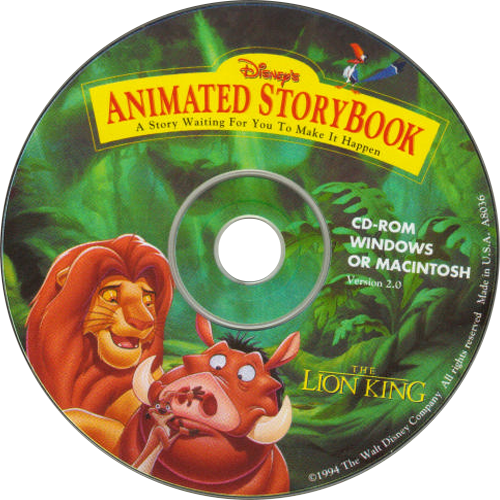
\includegraphics{lionking}
  % };
  \source{\cite{AnimatedStoryBook101}, \cite{AnimatedStoryBookWinnie},
    \cite{AnimatedStoryBookLion}, \cite{AnimatedStoryBookHercules},
    \cite{AnimatedStoryBookPocahontas}}
\end{frame}

\begin{frame}
  \fitimage{dalmatians-demo}
  \source{\cite{DisneyAnimatedStoryBook1996}, \cite{AnimatedStoryBook101}}
\end{frame}

\againframe{msitrans}

\begin{frame}
  \fitimage{overlay2.png}
  \source{\cite{AmazonComTonka}, \cite{AmazonComTonkab},
    \cite{AmazonComTonkaa}, \cite{PickyEaterPC}}
\end{frame}

% \begin{frame}
% \begin{center}
%   ``I lost my copy of the source many years ago when a backup drive failed. I was
%   hoping to do a similar thing to what ScummVM does...''
% \end{center}
% \end{frame}

\begin{frame}{Research Question}\pause
  \begin{center}
    \huge How can an interactive multimedia format be reverse engineered from scratch?
  \end{center}
\end{frame}

% To show how I have begun answering this question...

\begin{frame}{Reverse Engineering}\pause
  \begin{center}
    \Large In reverse engineering,\\ ``One attempts to understand \textbf{through deductive
    reasoning} how a [system] accomplishes a task with very little... insight into
    exactly how it does so.''
  \end{center}
  \source{\cite{ReverseEngineering2021}}
\end{frame}

\begin{frame}{Reverse Engineering Process}\pause
  \LARGE \tableofcontents[pausesections]
\end{frame}

\begin{frame}{Bytes}\pause
  \Large
\begin{itemize}
  \item \textbf{Base-10} (decimal) uses 10 digits --\pause{} the numbers 0-9.\\\pause
  \item \textbf{Base-2} (binary) uses 2 digits --\pause{} the bits \texttt{0} and \texttt{1}.\\\pause
  \item \textbf{Base-16} (hexadecimal) uses 16 digits --\pause{} the numbers 0-9\pause{} and
    \centerline{\LARGE \hspace{-2em} \textbf{letters \texttt{A}-\texttt{F}}.}
\end{itemize}
\end{frame}

\begin{frame}{Bytes}\pause
  \begin{center}
    \Large A \textbf{byte} is a collection of 8 bits.\\\pause
    Each byte represents a value from $0 = (2^0 - 1)$\pause{} to $255 = (2^8 - 1)$.\pause

    \vspace{1em}
    For example,\pause
    \begin{equation*}
      (10101010)_2\pause \equiv \mathbf{(AA)}_{16}\pause \equiv (170)_{10}.\pause
    \end{equation*}

    Additionally,\pause
    \begin{equation*}
      \mathbf{(AA)_{16}}\pause\equiv  \textbf{\texttt{0xAA}}\pause \equiv  \textbf{\texttt{0xaa}}.
    \end{equation*}
  \end{center}
\end{frame}

\section{Understand file formats}

\begin{frame}{Files}
  % https://tex.stackexchange.com/questions/23647/drawing-a-directory-listing-a-la-the-tree-command-in-tikz
  \begin{figure}
    \begin{forest}
      [DALMATIANS
      [DATA
      [BOOT.STM,name=boot]
      [100.CXT,name=startcxt] % Include dots here
      [101.CXT]
      [3983.CXT,name=endcxt]
      [PROFILE.\textunderscore ST]
      ] % Include dots here
      [101\textunderscore ASB.EXE]]
      \pause{}
      \node[draw,line width=1mm,fit={(startcxt) (endcxt)},label={[label
        distance=0.3cm]0:\huge Contexts}] {};
    \end{forest}
  \end{figure}
\end{frame}

\begin{frame}{Files}\pause
  \begin{center}
    \Large A \textbf{file} is a collection of bytes united under one name.\\\pause
    Each byte has a unique \textbf{address} -- its position in the file.\pause
  \end{center}\vspace{-1em}
  \begin{figure}
    \hexdump{garage-117-0x00-0x80.0}{garage}{117.cxt}
  \end{figure}
\end{frame}

\begin{frame}{Files}
  \begin{center}
    \Large A \textbf{file} is a collection of bytes united under one name.\\
    Each byte has a unique \textbf{address} -- its position in the file.
  \end{center}\vspace{-1em}
  \begin{figure}
    \hexdump{garage-117-0x00-0x80.1}{garage}{117.cxt}
  \end{figure}
\end{frame}

\begin{frame}{Files}
  \begin{figure}
    \hexdump{garage-117-0x00-0x80.1}{garage}{117.cxt}
  \end{figure}
  \begin{center}
    \Huge \texttt{RIFF}
  \end{center}
\end{frame}

\newcommand{\chunkbox}{
  \adjustbox{lap={\width}{1em}}{\bitbox{8}{Tag} \bitbox{8}{Size}}
}
\begin{frame}{\texttt{RIFF}}\pause
  \vspace{-1.5em}
  \begin{columns}
    \begin{column}{0.3\textwidth}
      \Huge \textbf{R}esource\\
      \textbf{I}nterchange \\
      \textbf{F}ile \\
      \textbf{F}ormat
    \end{column}\pause
    \begin{column}{0.7\textwidth}
      \begin{figure}
        \begin{bytefield}{16}
          \begin{leftwordgroup}[curlyspace=0.5em]{File}
            \bitbox{8}{Tag} \bitbox{8}{Size} \\
            \begin{rightwordgroup}[curlyspace=1em]{Chunk}
              \chunkbox \\
              \adjustbox{lap={\width}{1em}}{\wordbox{2}{Data}}
            \end{rightwordgroup} \\
            \wordbox[]{1}{{\adjustbox{lap={\width}{1em}}{\Huge $\vdots$}}}\vspace{0.5em} \\
            \begin{rightwordgroup}[curlyspace=1em]{Chunk}
              \chunkbox \\
              \adjustbox{lap={\width}{1em}}{\wordbox{2}{Data}}
            \end{rightwordgroup}
          \end{leftwordgroup}
        \end{bytefield}
      \end{figure}
    \end{column}
  \end{columns}
\end{frame}

\begin{frame}[fragile]{\texttt{RIFF}}
\begin{lstlisting}[firstnumber=1, label=glabels, xleftmargin=10pt]
typedef struct {
     char ckID[4];         // Unique chunk identifier
     uint32 ckSize;        // Size of field <ckData>
     byte *ckData[ckSize]; // Actual data
} chunk;
\end{lstlisting}
\end{frame}

\begin{frame}{Files}
  \begin{figure}
    \only<1-3>{\hexdump{garage-117-0x00-0x80.2}{garage}{117.cxt}}
    \only<4>{\hexdump{garage-117-0x00-0x80.3}{garage}{117.cxt}}
    \only<5>{\hexdump{garage-117-0x00-0x80.4}{garage}{117.cxt}}
  \end{figure}
  \begin{overlayarea}{\textwidth}{0.3\textheight}
    \only<1-4>{
      \begin{center}\pause
        \Huge \texttt{0x09\,c7\,66} bytes\\ \pause
        \huge \textbf{(little endian)}
      \end{center}
    }
    \only<5>{
      \begin{center}
        \Huge What's in there?\\
        \huge \textbf{\texttt{igod}?}
      \end{center}
    }
  \end{overlayarea}
\end{frame}

\section{Parse data structures}

\begin{frame}{Structures}\pause
  \fitimage{garage}
  \source{\cite{AmazonComTonka}}
\end{frame}

% Don't change the space with highlighting:
% https://tex.stackexchange.com/questions/198931/color-overshoots-when-using-cellcolor-without-intercolumn-space
\newcommand{\headerinternal}[4]{
  \begin{figure}
    \hexdump{#1.#2}{#3}{#4}
  \end{figure}
  \begin{textblock*}{1cm}(15cm,1.5cm)
    \tiny{Header: #1.#2}
  \end{textblock*}
}

\newcommand{\imageheader}[1]{
  \headerinternal{garage-117-0x2200-0xa0}{#1}{garage}{117.cxt}
}

\newcommand{\imagedata}[1]{
  \headerinternal{garage-117-0x4a80e-0x60}{#1}{garage}{117.cxt}
}

\begin{frame}[label=header]{Structures}
  \foreach\x in {0,1,2,3,4,5,6,7,8,9} {
    \pgfmathtruncatemacro{\jn}{\x+1}%
    \only<\jn>{\imageheader{\x}}
  }
  \only<11>{\imageheader{9}}
  \only<12-17>{\imageheader{10}}
  \only<18>{\imageheader{11}}
  \only<19>{\imageheader{12}}
  \only<20>{\imageheader{13}}
  \only<21-22,24-25>{\imageheader{14}}
  \only<23>{\imagedata{1}}

  \begin{overlayarea}{\textwidth}{0.2\textheight}
    \only<10-11>{
      \begin{center}
        \Huge \texttt{03 00}\only<11>{: \texttt{uint16}}
      \end{center}
    }
    \only<13>{
      \begin{center}
        \Huge \texttt{img_7xn1_background}
      \end{center}
    }
    \only<14>{
      \vspace{-1em}
      \begin{center}
        \Large \texttt{img_7xn1_background} \\
        \Huge $19\equiv \texttt{0x13}$
      \end{center}
    }
    \only<15-16>{
      \begin{center}
        \Huge \texttt{04 00}\only<16>{: \texttt{uint32}}
      \end{center}
    }
    \only<17>{
      \begin{center}
        \Huge \texttt{12 00}: \texttt{string}
      \end{center}
    }
    \only<22-24>{
      \begin{center}
        \Huge \texttt{a0a5}
      \end{center}
    }
    \only<25>{
      \begin{center}
        \Huge \texttt{1b 00}: \texttt{ref}
      \end{center}
    }
  \end{overlayarea}
\end{frame}

% \begin{frame}{Structures}
%   \begin{figure}
%     \begin{forest}
%       [100.CXT
%       [RIFF
%       [igod] % Include dots here
%       [a001]] % Include dots here
%       [RIFF
%       [a100]] % Include dots here
%       [RIFF
%       [a200]]]
%     \end{forest}
%   \end{figure}
% \end{frame}

\begin{frame}[fragile]{Structures}\pause
  \begin{center}
    \Large \textbf{datum}\pause{} (data):\pause{} a single piece of information.\pause
  \end{center}
\begin{lstlisting}
class DatumType(IntEnum):
    UINT8      = 0x0002,
    UINT16     = 0x0003,
    SINT16     = 0x0010,
    STRING     = 0x0012,
    FILE       = 0x000a,
    POINT      = 0x000f,
    REF        = 0x001b,
    BBOX       = 0x000d,
    POLY       = 0x001d
\end{lstlisting}
\end{frame}

\begin{frame}[fragile]{Structures}
  \begin{center}
    \Large \textbf{datum} (data): a single piece of information.
  \end{center}
\begin{lstlisting}
class DatumType(IntEnum):
    UINT8      = 0x0002,
    UINT16     = 0x0003,
    SINT16     = 0x0010,
    STRING     = 0x0012,
    FILE       = 0x000a,
    (*\LARGE \verb|POINT   = 0x000f|*),
    REF        = 0x001b,
    BBOX       = 0x000d,
    POLY       = 0x001d
\end{lstlisting}
\end{frame}

\begin{frame}[label=proverb]{Structures}
  \begin{center}
    \LARGE In reverse engineering, your discoveries unexpectedly build upon themselves.
  \end{center}
\end{frame}

\newcommand{\ThoughtProcess}{
  \begin{center}
    \large ``Background'' $\implies$ Full-screen $\implies$ VGA Graphics $\implies$
    $640\times 480$
  \end{center}
}
\begin{frame}<1-11>[label=discover1]{Structures}
  \only<1-7>{\imageheader{0}}
  \only<8>{\imageheader{15}}
  \only<9-10>{\imageheader{16}}
  \only<11>{\imageheader{17}}
  \only<12>{\imageheader{18}}
  \only<13-15>{\imageheader{20}}
  \begin{center}\pause
    \Large ``Background''\pause{} $\implies$\pause{} Full-screen $\implies$\pause{} VGA Graphics $\implies$\pause{}
    $640\times 480$
  \end{center}\pause\vspace{-1em}
  \begin{overlayarea}{\textwidth}{0.2\textheight}
  \only<1-8>{
    \begin{center}
      \Huge $640\equiv \texttt{0x02\,80} \equiv \texttt{08 20}$
    \end{center}
  }
  \only<9-10>{
    \begin{center}
      \only<10>{\Huge $480\equiv \texttt{0x01\,e0} \equiv \texttt{e0 01}$}
    \end{center}
  }
  \only<11-12>{
    \begin{center}
      \LARGE \textbf{Point}: $(x, y)$
    \end{center}
  }
  \only<13,15>{
    \begin{center}
      \LARGE $(0, 0)$;\pause{} $(640, 480)$
    \end{center}
  }
  \only<14>{
    \begin{center}
      \LARGE \textbf{Bounding box}: left, top; width, height.
    \end{center}
  }
\end{overlayarea}
\end{frame}

\againframe{proverb}

\againframe<11->{discover1}

\newcommand{\soundheader}[1]{
  \headerinternal{garage-117-0x2c26-0x72}{#1}{garage}{117.cxt}
}

% \begin{frame}{Structures}
%   \soundheader{0}
% \end{frame}

\begin{frame}
  % \fitimage{cxtcode}
  \vspace{-1em}
  \begin{figure}
    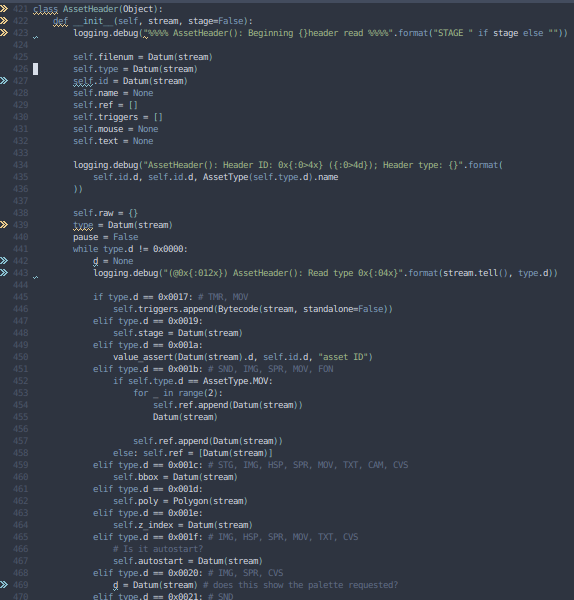
\includegraphics[height=\textheight]{cxtcode}
  \end{figure}
\end{frame}

\begin{frame}
  \fitimage{cxtrepo}
\end{frame}

\begin{frame}[fragile]{Structures}
\begin{lstlisting}[basicstyle=\ttfamily\small]
  "header": {
    "filenum": 117,
    "type": 7,
    "id": 300,
    "name": "img_7xn1_background",
    "ref": ["a0a5"],
    (*\tikzmark{a}*)"bbox": {
      "point": {
        "x": 0,
        "y": 0
      },
      "dims": {
        "x": 640,
        "y": 480
      }
    },(*\tikzmark{b}*)
    "z_index": 32000
  }
\end{lstlisting}
  \only<2>{
  \begin{tikzpicture}[remember picture,overlay]
    \draw[red,rounded corners]
     ([shift={(-1em,1em)}]pic cs:a)
     rectangle
     ([shift={(8em,-0.3em)}]pic cs:b);
  \end{tikzpicture}}%
\end{frame}

\section{Extract game assets}

\begin{frame}{Assets}
  \only<1>{\imageheader{0}}
  \only<2-3>{\imageheader{6}}
  \begin{overlayarea}{\textwidth}{0.2\textheight}
    \only<3>{\vspace{-1em}
      \begin{center}
      \Huge \texttt{07 00}
    \end{center}}
  \end{overlayarea}
\end{frame}

\begin{frame}[fragile]{Assets}
\begin{lstlisting}
class AssetType(IntEnum):
    SCR  = 0x0001, # Screen
    STG  = 0x0002, # Stage
    PTH  = 0x0004, # Path
    SND  = 0x0005, # Sound
    TMR  = 0x0006, # Timer
    IMG  = 0x0007, # Image
    HSP  = 0x000b, # Hotspot
    SPR  = 0x000e, # Sprite
    MOV  = 0x0016, # Movie
    PAL  = 0x0017, # Palette
    FON  = 0x001b, # Font
    FUN  = 0x0069, # Function
\end{lstlisting}
\end{frame}

\begin{frame}{Assets}
  \foreach\x in {0,1,2,3}{
    \only<\x>{\imagedata{\x}}
  }
  \only<4-5>{\imagedata{4}}
  \only<6>{\imagedata{5}}
  \only<7>{\imagedata{6}}
  \begin{overlayarea}{\textwidth}{0.3\textheight}
    \only<5-7>{
      \begin{center}
        \huge $640 \times 480 = 307\,200 \equiv \texttt{0x4b000}$ \\
        \only<6-7>{$\texttt{00 b0 04 00}$}
      \end{center}
    }
  \end{overlayarea}
\end{frame}

\begin{frame}{Assets}
  \fitimage{300.png}
\end{frame}

\newcommand{\rledata}[1]{
  \headerinternal{garage-110-0x4b9f4-0x60}{#1}{garage}{110.cxt}
}

\begin{frame}<-6>[label=assets]{Assets}
  \foreach\x in {0,1,2,3}{
    \only<\x>{\rledata{\x}}
  }
  \only<4-7>{\rledata{4}}
  \only<8-11>{\rledata{5}}
  \only<12>{\rledata{6}}
  \only<13-14>{\rledata{7}}
  \only<15>{\rledata{8}}
  \only<16>{\rledata{9}}
  \only<17-18>{\rledata{10}}
  \begin{overlayarea}{\textwidth}{0.3\textheight}
    \vspace{-1em}
    \only<5-6>{
      \begin{figure}
        
\includegraphics{bad}
      \end{figure}
    }
    \only<6>{
      \vspace{-1.5em}
      \begin{center}
        \LARGE $\texttt{0x00f8} \times \texttt{0x00c9} = \texttt{0xc2b8} > \texttt{0x298e}$
      \end{center}
    }
    \only<7-8>{
      \begin{figure}
        
\includegraphics[height=0.2\textheight]{flagtop}
      \end{figure}
    }
    \only<9>{
      \begin{figure}
        
\includegraphics[height=0.2\textheight]{flagtop1}
      \end{figure}
      \vspace{-2em}
      \begin{center}
        \Huge $17\equiv \texttt{0x11}$ pixels wide
      \end{center}
    }
    \only<10>{
      \begin{table}
        \LARGE
        \begin{tabular}{c@{ }|@{ }c@{ }|@{ }c@{ }|@{ }c@{ }|@{ }c@{ }}
          \texttt{00 00} & \texttt{00 03} & \texttt{78 00} & \texttt{11} & \texttt{fe} \\
          \hline
          New row & Encoding & Offset & Run length & Color
        \end{tabular}
      \end{table}
    }
    \only<11,18>{
      \vspace{2em}
      \begin{center}
        \Huge \textbf{R}un \textbf{L}ength \textbf{E}ncoding \Large (\textbf{RLE})
      \end{center}
    }
    \only<12>{
      \begin{table}
        \LARGE
        \begin{tabular}{c@{ }|@{ }c@{ }|@{ }c@{ }|}
          \texttt{00 00} & \texttt{00 03} & \texttt{76 00} \\
          \hline
          New row & Encoding & Offset
        \end{tabular}
      \end{table}
    }
    \only<13>{
      \begin{figure}
        
\includegraphics[height=0.2\textheight]{flagtop2}
      \end{figure}
    }
    \only<14>{
      \begin{table}
        \LARGE
        \begin{tabular}{c@{ }|@{ }c@{ }|}
          \texttt{00 04} & \texttt{fe fe fe 55} \\
          \hline
          Raw length & Data
        \end{tabular}
      \end{table}
    }
    \only<15>{
      \begin{figure}
        
\includegraphics[height=0.2\textheight]{flagtop3}
      \end{figure}
    }
    \only<16>{
      \begin{figure}
        
\includegraphics[height=0.2\textheight]{flagtop4}
      \end{figure}
    }
    \only<17>{
      \begin{figure}
        
\includegraphics[height=0.2\textheight]{flagtop5}
      \end{figure}
    }
  \end{overlayarea}
\end{frame}

\begin{frame}{Assets}
  % \fitimage{172}
  \begin{figure}
    \only<1>{
\includegraphics{172}}
    \only<2>{
\includegraphics{flagtop}}
  \end{figure}
\end{frame}

\againframe<7->{assets}

\begin{frame}
  \vspace{-1em}
  \begin{figure}
    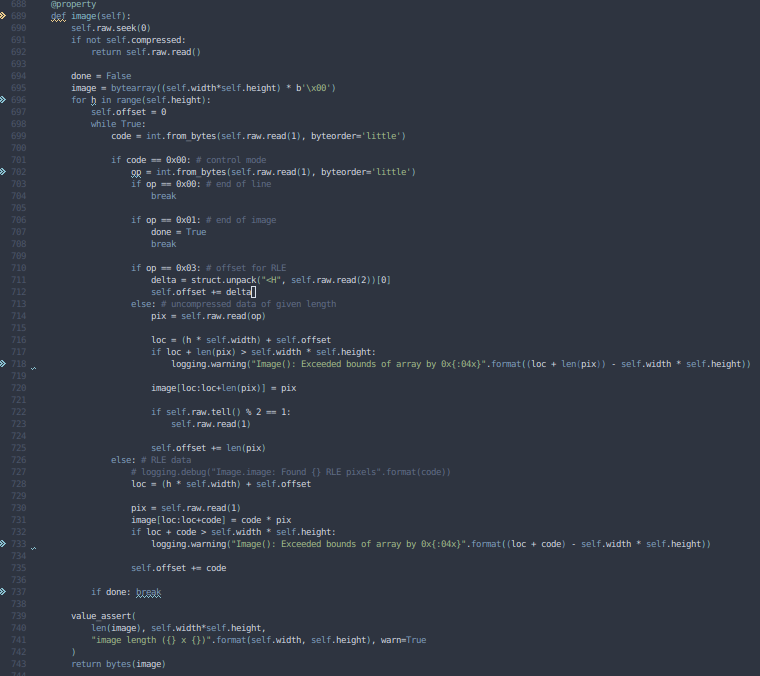
\includegraphics[height=\textheight]{imagecode}
  \end{figure}
\end{frame}

\begin{frame}
  \begin{figure}
    
\includegraphics[height=\textheight]{85-0}
  \end{figure}
\end{frame}

\begin{frame}{Assets}
  \Large We haven't even begun discussing...
  \begin{itemize}
    \item Decoding sounds\pause
    \item Extracting animation sequences\pause
    \item Handling fonts and text\pause
    \item Decompiling game bytecode
  \end{itemize}
\end{frame}

\section{Write interactive engine}

\newcommand{\bcdata}[1]{
  \headerinternal{dalmatians-168-0x4b7c-0x94}{#1}{dalmatians}{168.cxt}
}

\begin{frame}[label=current,fragile]{Code}
  % \vspace{-1em}
  % \begin{center}
  %   \huge Code
  % \end{center}
\begin{lstlisting}
class Movie(Object):
    def __init__(self, stream, header, chunk, stills=[]):
        self.stills = stills
        self.chunks = []

        end = stream.tell() + chunk['size']
        codes = {
            "header": chunk_int(chunk),
            "video" : chunk_int(chunk) + 1,
            "audio" : chunk_int(chunk) + 2,
        }
\end{lstlisting}
\end{frame}

\begin{frame}{Bytecode}
  \bcdata{0}
\end{frame}

\begin{frame}
  \begin{center}
    \LARGE In bytecode, \\
    \textbf{numbers take the place of words}.\pause
  \end{center}
  \begin{table}
    \Large \begin{tabular}{@{ }c@{ }|@{ }c@{ }}
      \textbf{Compile} \onslide<3>{& \textbf{Decompile}} \\
      \hline
      \texttt{Code}$\implies$ Bytecode \onslide<3>{& Bytecode $\implies$ \texttt{Code}}
    \end{tabular}
  \end{table}
\end{frame}

\begin{frame}[label=func]{Interactivity}
    \only<2>{\bcdata{0}}
    \only<3>{\bcdata{1}}
\end{frame}

\begin{frame}[fragile]{Interactivity}
  \vspace{-3em}
  \begin{center}
    \begin{tabular}{c}
\begin{lstlisting}[basicstyle=\fontsize{8}{9}\selectfont]
{
  "sz": 114,
  "ch": [
    {
      "sz": 108,
      "ch": [
        [
          202,
          [207, [103], 4],
          [156, 0]
        ],
        {
          "sz": 20,
          "ch": [
            [
              219, 119, 0
            ],
            0
          ]
        },
        [220, 202, 0],
        [103],
      ]
    }
  ]
}
\end{lstlisting}
    \end{tabular}
\end{center}
\end{frame}

\begin{frame}{Pseudocode}\pause
  \begin{enumerate}
    \LARGE
  \item \texttt{``Display asset 119.''}\pause
  \item \texttt{``When asset 119 is clicked, play movie 202 at its location.''}\pause
  \item \texttt{``When movie 202 finishes, play asset 120.''}\pause
  \end{enumerate}
\end{frame}

\againframe<2>{func}

\begin{frame}
  \fitimage{scummvm}\pause
  \begin{center}
    \Huge To be continued...
  \end{center}
  \source{\cite{ScummVM}}
\end{frame}

\frame{\titlepage}

% Info about the bytecode

% Repeat the title slide

\begin{frame}[allowframebreaks]{References}
  \bibliographystyle{IEEEtran}
  \bibliography{MediaStation}
\end{frame}
\end{document}
